%Appendix -- January 2015
\appendix
\renewcommand{\thechapter}{B}
\renewcommand{\chaptername}{Appendix}

\chapter{RbLi: the good, the bad and the ugly}
\label{app:RbLi}

\begin{figure*}[htb]
\begin{center}
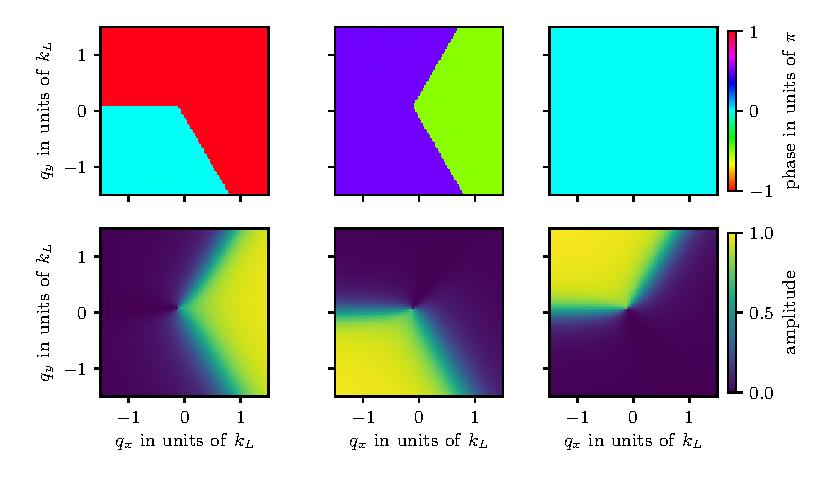
\includegraphics[]{Figures/Chapter8/topological_eigenvecs.pdf}
\caption{{\bfseries a} Probabilities as a function of quasimomentum for the three output ports of the interferometer at $t_{\rm free}=\unit[160]{\mu s}$ {\bfseries b} Probabilities as a function of free evolution time $t_{\mathrm{free}}$ for an input state with quasimomentum $(q_1, q_2)=(0.55,-0.92)\,k_{\rm L}$ indicated by the blue star on {\bfseries a} and in the topological ground branch ($n=1$)}
\label{fig:topological_eigenvecs}
\end{center}
\end{figure*}

\begin{figure*}[htb]
\begin{center}
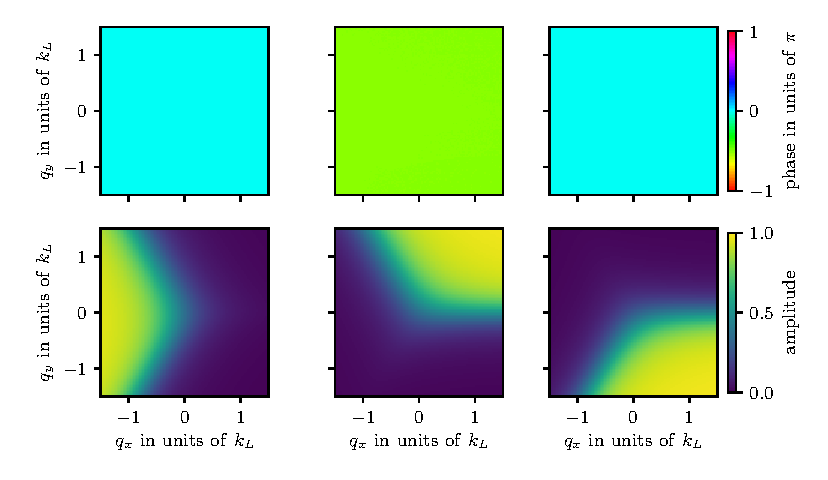
\includegraphics[]{Figures/Chapter8/nontopological_eigenvecs.pdf}
\caption{{\bfseries a} Probabilities as a function of quasimomentum for the three output ports of the interferometer at $t_{\rm free}=\unit[160]{\mu s}$ {\bfseries b} Probabilities as a function of free evolution time $t_{\mathrm{free}}$ for an input state with quasimomentum $(q_1, q_2)=(0.55,-0.92)\,k_{\rm L}$ indicated by the blue star on {\bfseries a} and in the topological ground branch ($n=1$)}
\label{fig:nontopological_eigenvecs}
\end{center}
\end{figure*}


\section{Water cooling stuff}
\section{Electrical installation}
\section{New Rb `oven'}

